\chapter{CHAPTER THREE: A Microstructure PDE } \label{chapter_3}

\section{Introduction}

One dimensional wave propagation in microstructured solids is currently a topic of great interest.
This phenomenon has recently been modeled \cite{STE} by an equation

\begin{equation}\label{eq:MS}
v_{tt} - b v_{xx} - \frac{\mu}{2} \left( v^2 \right)_{xx} - \delta \left( \beta v_{tt} - \gamma v_{xx}\right)_{xx} = 0 
\end{equation}
with complicated dispersive and nonlinear terms. Here $b, \mu, \beta, \delta$
and $\gamma$ are dimensionless parameters, $v$ denotes the macrodeformation,
and $x$ and $t$ denote space and time coordinates respectively.

Equation \eqref{eq:MS} is derived, using the so-called Mindlin Model, in
\cite{STE}, \cite{JE1}, \cite{JE2}.  It is non-integrable. However, analytic
conditions for the existence of solitary waves of \eqref{eq:MS} have been
derived in \cite{JE2} and \cite{STE}. These references also numerically
construct asymmetric solitary wave solutions of the form $ v\left(x - c t
\right)$ of \eqref{eq:MS}.  More recently (\cite{EP},\cite{EBS}) pulse trains
in \eqref{eq:MS} have been numerically constructed.

\section{Solitary waves; local bifurcations}


Solitary waves of \eqref{eq:MS} of the form 
$v(x,t) = \phi\left(x - c t\right) = \phi\left(z\right)$
 satisfy the fourth-order traveling wave ODE
\begin{equation} \label{eq:ode2} \phi_{zzzz} - q \phi_{zz} + p \phi = \mathcal{N}[\phi]
\end{equation}

where 
\begin{equation}
\mathcal{N}\left[\phi\right] = -\Delta_1 \phi_z^2 - b \Delta_1 \phi \phi_{zz}
\end{equation}
and
\begin{subequations}
\begin{eqnarray}
z &\equiv& x - c t\\
p &\equiv& 0\label{eq:pdef} \\
q &\equiv & \frac{c^2 - b}{\delta\left(\beta c^2 - \gamma\right)} 
\label{eq:qdef2} \\
\Delta_1 &\equiv& \frac{\mu}{ \delta\left( \beta c^2 - \gamma\right) }\label{eq:deltadef} 
\end{eqnarray}
\end{subequations}
Equation \eqref{eq:ode2} is invariant under the transformation $ z \mapsto -z $ and is thus a reversible system. In this section we shall
use the theory of reversible systems to characterize the homoclinic orbits to the fixed point of \eqref{eq:ode2}, which correspond to pulses
or solitary waves of \eqref{eq:MS} in various regions of the $(p,q)$ plane.

The linearized system corresponding to \eqref{eq:ode2}
\begin{equation}
 \label{eq:linode2} \phi_{zzzz} - q \phi_{zz} + p \phi = 0
\end{equation}
has a fixed point \begin{equation}\label{eq:fp2} \phi = \phi_z = \phi_{zz} = \phi_{zzz} = 0 \end{equation}

Solutions $\phi = k e^{\lambda x}$ satisfy the characteristic equation
$\lambda^4 - q \lambda^2 + p = 0 $ from which one may deduce that the structure
of the eigenvalues is distinct in two regions of $\left(p,q\right)$-space.
Since $p=0$ we have only two possible regions of eigenvalues.  We denote $C_0$
as the positive $q$ axis and $C_1$ the negative $q$-axis. First we shall 
consider the bounding curves $C_0$ and $C_1$ and their neighborhoods, then we shall discuss the possible
occurrence and multiplicity of homoclinic orbits to \eqref{eq:fp2}, corresponding
to pulse solitary waves of \eqref{eq:MS}, in each region:

\begin{description}
\item[Near $C_0$] 
The eigenvalues have the structure $\lambda_{1-4} = 0,0,\pm \lambda$, ($\lambda \in \mathbb{R}$) and the fixed point
\eqref{eq:fp} is a saddle-focus.
\item[Near $C_1$] 
Here the eigenvalues have the structure $\lambda_{1-4} = 0,0,\pm i \omega $, ($\omega \in \mathbb{R}$) . We will show by analysis of a
four-dimensional normal form in Section 4 that there exists a $\mathrm{sech}^2$ homoclinic orbit near $C_1$.
\end{description}

Having outlined the possible families of orbits homoclinic to the fixed point \eqref{eq:fp2} of \eqref{eq:linode2},
corresponding to pulse solitary waves of \eqref{eq:MS}, we now derive normal forms near the transition curves $C_0$ and $C_1$
to confirm the existence of regular or delocalized solitary waves in the corresponding regions of $\left(p,q\right)$ parameter space.

\section{Normal form near $C_0$: solitary wave solutions}

Using \eqref{eq:linode2}, the curve $C_0$, corresponding to $\lambda = 0,0,\pm \tilde{ \lambda } $, is given by
\begin{equation}
C_0: { p=0, q > 0 }
\end{equation}

Using \eqref{eq:qdef2} implies
\begin{equation}
 \frac{c^2 - b}{\delta\left(\beta c^2 - \gamma\right)} > 0
\end{equation}

Denoting $\phi$ by $y_1$, equation \eqref{eq:ode2} may be written as the system
\begin{subequations}\label{eq:system2}
\begin{eqnarray}
\frac{d y_1 }{d z} &=& y_2 \\
\frac{d y_2 }{d z} &=& y_3 \\
\frac{d y_3 }{d z} &=& y_4 \\
\frac{d y_4 }{d z} &=& q y_3 - p y_1 - \left(\Delta_1 y_2^2 + b \Delta_1 y_1 y_3 \right)
\end{eqnarray}
\end{subequations}

We wish to rewrite this as a first order reversible system in order to invoke the relevant theory \cite{IA}. 
To that end, defining  $Y=\left<y_1,y_2,y_3,y_4\right>^T$, equation \eqref{eq:system2} may be written 

\begin{equation}\label{eq:bilinearms}
\frac{ dY }{ dz } = L_{pq} Y - F_2(Y,Y)
\end{equation}

where 
\begin{equation}
L_{pq} = \left( 
\begin{array}{cccc}
0&1&0&0\\
q/3&0&1&0\\
0&q/3&0&1\\
q^2 - p &0&q/3&0 \end{array} \right) \end{equation}

Since $p=0$ for \eqref{eq:MS}, we have 
\begin{equation} \label{eq:bilinearms2}
 \frac{ dY }{ dz } = L_{0q} Y - F_2(Y,Y) 
\end{equation}
where 
\begin{equation}\label{eq:nonlinear2}
F_2(Y,Y) = \left<0,0,0,\Delta_1 y_2^2 + b \Delta_1 y_1 y_3 \right>^T
\end{equation}

Next we calculate the normal form of \eqref{eq:bilinearms2} near $C_0$. The procedure is
closely modeled on \cite{IA} and many intermediate steps may be found there. 

\subsection{ Near $C_0$ }
Near $C_0$ the dynamics reduce to a two-dimensional Center Manifold
\begin{equation}\label{eq:c0cm2}
 Y = A \zeta_0 + B \zeta_1 + \Psi(\epsilon,A,B)
\end{equation}
and the corresponding normal form is
\begin{subequations}\label{eq:c0nf2}
\begin{eqnarray}
\frac{dA}{dz} &=& B \label{eq:c0nf2a} \\
\frac{dB}{dz} &=& b \epsilon A + \tilde{c} A^2 \label{eq:c0nf2b}
\end{eqnarray}
\end{subequations}
Here,
\begin{equation}
\epsilon = \left( \frac{q^2}{9} - p\right) - \left(\frac{q}{3}\right)^2 = - p 
\end{equation}
measures the perturbation around $C_0$, and
\begin{subequations}\label{eq:lineareigs2}
\begin{eqnarray}
\zeta_0 &=& \left<1,0,-q/3,0\right>^T\\
\zeta_1 &=& \left<0,1,0,-2 q/3\right>^T 
\end{eqnarray}
\end{subequations}

The linear eigenvalue of \eqref{eq:c0nf2} satisfies 
\begin{equation}\label{eq:lineig2}
\lambda^2 = b \epsilon 
\end{equation}
The characteristic equation of the linear part of 
\eqref{eq:bilinearms2} is 
\begin{equation}\label{eq:charlinear2}
\lambda^4 - q \lambda^2 - \epsilon =  0 
\end{equation}
Hence, the eigenvalues near zero (the Center Manifold) satisfy $\lambda^4 \ll \lambda^2$ and hence 
\begin{equation}\label{eq:lindominant2}
\lambda^2 \sim -\frac{\epsilon}{q}
\end{equation}
Matching \eqref{eq:lineig2} and \eqref{eq:lindominant2} 
\begin{equation}
b = - \frac{1}{q}
\end{equation}
and only the nonlinear coefficient $\tilde{c}$ remains to be determined in the normal form \eqref{eq:c0nf2}.

In order to determine $\tilde{c}$ (the coefficient of $A^2$ in \eqref{eq:c0nf2})
we calculate $\frac{dY}{dz}$ in two ways and match the $\mathcal{O}(A^2)$
terms.  To this end, using the standard 'suspension' trick of treating the
perturbation parameter $\epsilon$ as a variable, we expand the function $\Psi$
in \eqref{eq:c0cm2} as 
\begin{equation}\label{eq:psiexpms}
\Psi(\epsilon,A,B) = \epsilon A \Psi_{10}^1 + \epsilon B \Psi_{01}^1 + A^2 \Psi_{20}^0 + A B \Psi_{11}^0 + B^2 \Psi_{02}^0 + \cdots
\end{equation}
where the subscripts denote powers of $A$ and $B$, respectively, and the superscript denotes the power of $\epsilon$. 

In the first way of computing $dY/dz$, we take
the $z$ derivative of \eqref{eq:c0cm}
\begin{equation}
\frac{dY}{dz} = B \zeta_0 + \left(b \epsilon A + \tilde{c} A^2\right)\zeta_1 + \frac{d\Psi}{dz}
\end{equation}
And finally using \eqref{eq:psiexpms} and \eqref{eq:c0nf2} again we arrive at
\begin{align}
\frac{dY}{dz} = B \zeta_0 + \left(b \epsilon A + \tilde{c} A^2\right)\zeta_1 + \left( b \epsilon^2 A + \epsilon \tilde{c} A^2\right) \label{eq:longeqn1}\\
                + 2 A B\Psi_{20}^0 + \left( B^2 + b\epsilon A^2 + \tilde{c} A^3\right)\Psi_{11}^0 \notag \\ 
                + 2 B \left( b \epsilon A + \tilde{c} A^2 \right)\Psi_{02}^0 + \cdots \notag
\end{align}



The coefficient of $A^2$ in the resulting expression is $\tilde{c} \zeta_1 $. In the second way of computing $dY/dz$, we use \eqref{eq:c0cm2} and \eqref{eq:psiexpms} in \eqref{eq:bilinearms2}. The coefficient of $A^2$ in the resulting expression is 
$ L_{0,q} \Psi_{20}^0 - F_2\left(\zeta_0,\zeta_0\right)$,
which leads to 
\begin{equation}\label{eq:A2coef2}
 \tilde{c} \zeta_1 = L_{0q} \Psi_{20}^0 - F_2(\zeta_0,\zeta_0) \end{equation}

Using \eqref{eq:lineareigs2} and \eqref{eq:nonlinear2} and denoting $\Psi_{20}^0 = \left<x_1,x_2,x_3,x_4\right>$ in \eqref{eq:A2coef2} yields the equations
\begin{subequations}
\begin{eqnarray}
0 &=& x_2 \\
\tilde{c} &=& \frac{q}{3} x_1 + x_3 \label{eq:A2coef2b}\\
0 &=& \frac{q}{3} x_2 + x_4 \implies x_4 = 0
\textrm{ using \eqref{eq:A2coef2b} }
\end{eqnarray}
\end{subequations}
and
\begin{equation}
-\frac{2q}{3} \tilde{c} = \frac{q}{3}\left(\frac{q}{3} x_1 + x_3 \right) + \frac{2q}{3} = \frac{q}{3} \tilde{c} + \frac{b \Delta_1 }{3} 
\textrm{ using \eqref{eq:A2coef2b} }
\end{equation}
Hence we obtain 
\begin{equation}
\tilde{c} = - \frac{b \Delta_1}{3} 
\end{equation}
 
Therefore, the normal form for \eqref{eq:MS} near $C_0$ is
\begin{subequations}\label{eq:msnf}
\begin{eqnarray}
\frac{dA}{dz} &=& B \label{eq:msnfa} \\
\frac{dB}{dz} &=& -\frac{\epsilon}{q} A - \frac{ b \Delta_1}{3}  A^2
\end{eqnarray}
\end{subequations}

The normal form \eqref{eq:msnf} admits a homoclinic solution (near $C_0$) of the form 
\begin{equation} \label{eq:ms_soliton1}
A\left(z\right) = \ell \space \mathrm{sech}^2\left(k z\right)
\end{equation}

To determine $k$ and $\ell$ we put \eqref{eq:ms_soliton1} into the equivalent second order equation for \eqref{eq:msnf},
$ \frac{dA^2}{dz^2} = -\frac{\epsilon}{q} A - \frac{b \Delta_1}{3} A^2 $. which implies
\begin{subequations}
\begin{eqnarray*}
\ell \left( - 2 k^2 \mathrm{sech}^4(kz) + 4 k^2 \mathrm{sech}^2(kz) \mathrm{tanh}^2(kz) \right) &=& -\frac{\epsilon}{q} \ell \mathrm{sech}^2(kz) - \frac{b \Delta_1}{3} \ell^2 \mathrm{sech}^4(kz) \\
4 k^2 \mathrm{sech}^2(kz) - 6 k^2 \mathrm{sech}^4(kz) &=& -\frac{\epsilon}{q} \mathrm{sech^2}(kz) - \frac{b \Delta_1}{3} \ell \mathrm{sech}^4(kz)
 \end{eqnarray*}
\end{subequations}
where we have used the same hyperboic identities as in Chapter 2.  
Matching the $\mathcal{O}(\mathrm{sech}^2(kz)$ and $\mathcal{O}(\mathrm{sech}^2(kz)$ terms on each side of the preceding equation implies
\begin{subequations}
\begin{eqnarray}
4k^2 = \frac{-\epsilon}{4q} &\implies& k = \sqrt{\frac{-\epsilon}{4q}}  \\
6 k^2 =  \frac{b \Delta_1}{3} \ell &\implies& \ell = \frac{18 k^2}{ b \Delta_1 }
 \end{eqnarray}
\end{subequations}

Hence, since $\epsilon = - p $, and the curve $C_0$ corresponds to $p=0,q>0$, solitary waves of the 
form \eqref{eq:ms_soliton1} exist in the vicinity of $C_0$ for 
\begin{equation}
p > 0, q > 0 
\end{equation}
which implies that $  \frac{c^2 - b}{\delta\left(\beta c^2 - \gamma\right)} > 0 $
(such that $k$  is real.)  As mentioned in section 2, one may show the persistence
of this homoclinic solution in the original traveling wave ODE \eqref{eq:linode2}. Thus, we have 
demonstrated the existence of solitary waves of \eqref{eq:MS} for $p=0^+, q>0$. 

\section{Normal form near $C_1$: possible solitary wave solutions}
Using \eqref{eq:linode2}, the curve $C_1$, corresponding to $\lambda = 0, 0\pm i \omega$, is given by
\begin{equation}\label{eq:ms_c1}
C_1 : { p = 0, q < 0 }
\end{equation}
Which implies
\begin{equation}
\frac{c^2 - b}{ \delta\left(\beta c^2 - \gamma \right)} < 0
\end{equation}

In order to investigate the possibility of a $ \mathrm{sech}^2 $  homoclinic orbit in
the neighborhood of $C_1$ and delocalized solitary waves, we next compute the
normal form near $C_1$ following the procedure in \cite{IA}.

Near $C_1$ the dynamics reduce to a four-dimensional Center Manifold \cite{IA}.
Since all the eigenvalues are non-hyperbolic, the Center Manifold has the form
(a nonlinear coordinate change \cite{IA})
\begin{equation} \label{eq:c1cm2}
Y = A \zeta_0 + B \zeta_0 + C \zeta_+ + \bar{C} \zeta_- + \Psi(\epsilon,A,B,C,\bar{C})
\end{equation}

with  a corresponding four-dimensional normal form
\begin{subequations}\label{eq:c1nf2}
\begin{eqnarray}
\frac{dA}{dz} &=& B \label{eq:aq2} \\
\frac{dB}{dz} &=& \bar{\nu} A + b_* A^2 + c_* \left|C\right|^2  \label{eq:bq2} \\
\frac{dC}{dz} &=& i d_0 C + i \bar{\nu} d_1 C + i d_2 A C \label{eq:cq2}
\end{eqnarray}
\end{subequations}
Here $C$ is complex, $\bar{C}$ is the complex conjugate of $C$, $\epsilon,
\zeta_0, \zeta_1$ are given previously and the two new complex eigenvectors
co-spanning the Center Manifold are
\begin{equation}
\zeta_\pm	 = \left< 1, \lambda_\pm, 2 q / 3, \frac{\lambda_\pm}{3} q\right>^T 
\end{equation}

Using \eqref{eq:bq2} and \eqref{eq:c0nf2b}
\begin{equation}
\bar{\nu} = b \epsilon = -\frac{\epsilon}{q} 
\end{equation}

Also from the characteristic equation \eqref{eq:charlinear2}, the two non-zero 
(imaginary) roots are 
\begin{equation}
\lambda^2 = \frac{ q + \sqrt{q^2 + 4 \epsilon } }{2} \approx q \textrm{ for } \epsilon \textrm{ small }
\end{equation}

Hence
\begin{equation}
\lambda = \pm i \sqrt{-q}, q < 0
\end{equation}

Matching this to the linear part of \eqref{eq:cq2} 
(which corresponds to the
imaginary eigenvalues), $\lambda = i d_0 = i \sqrt{-q}$ or 
\begin{equation}
d_0 = \sqrt{-q}
\end{equation}

With a dominant balance argument on the characteristic equation \eqref{eq:charlinear2} as  $\lambda \rightarrow \pm i \sqrt{-q}$ we find
\begin{equation}
d_1 = \frac{\sqrt{-q}}{2 q^2} 
\end{equation}


The remaining undetermined coefficients  in the normal form are the 
coefficients $b_*,c_*$ and $d_2$ 
which correspond to the $A^2, |C|^2$ and $AC$ terms respectively. In 
order to determine them, we follow the same procedure as 
in Section 3 and compute $dY/dz$ is two distinct ways. We expand the
function $\Psi$ as
\begin{equation}\label{eq:psiexpms2}
\Psi(\epsilon,A,B,C,\bar{C}) = \epsilon A \Psi_{1000}^1 + \epsilon B \Psi_{0100}^1 + A^2 \Psi_{2000}^0 + A B \Psi_{1100}^0 + A C \Psi_{1010}^0 + \epsilon C \Psi_{0010}^1 + \cdots 
\end{equation}

with subscripts denoting powers of $A$, $B$, $C$ and $\bar{C}$, respectively,
and the superscript is the power of $\epsilon$. In the first way, $dY/dz$ is
computed by taking the $z$ derivative of \eqref{eq:c1cm2} (using \eqref{eq:c1nf2}
and \eqref{eq:psiexpms2}) and read off the coefficients of $A^2, \|C\|^2, C
\epsilon$ and $AC$ terms.  In the second way, $dY/dz$ is computed using
\eqref{eq:c1cm2} and \eqref{eq:psiexpms2} in \eqref{eq:bilinearms2} (with $p=0$ on
$C_1$ as given in \eqref{eq:ms_c1}) and the coefficients of  $A$, $B$, $C$ and
$\bar{C}$ are once again read off.  Equating the coefficients of the
corresponding terms in the two separate expressions for $dY/dz$ yields the
following equations:
\begin{subequations}
\begin{eqnarray}
\mathcal{O}(A^2): &		b_* \zeta_1 &= L_{0q} \Psi_{2000}^0 - F_2(\zeta_0,\zeta_0) \\
\mathcal{O}(\left|C\right|^2):&	c_* \zeta_1 &= L_{0q} \Psi_{0011}^0 -2 F_2(\zeta_+,\zeta_-) \label{eq:cstar2} \\
\mathcal{O}(\epsilon C): &-\frac{i}{q} \left(d_1 \zeta_+ +  d_0 \Psi_{0010}^1\right) &= L_{0q} \Psi_{0010}^1 \\
\mathcal{O}(A C): 	&i d_2 \zeta_+ + i d_0 \Psi_{1010}^0 &= L_{0q} \Psi_{1010}^0 - 2 F_2(\zeta_0,\zeta_+) \label{eq:AC2}
\end{eqnarray}
\end{subequations}
where we have used the fact that $F_2(Y,Y)$ is a symmetric bilinear form. We would like to evaluate $F_2\left(\zeta_+, \zeta_-\right)$, so we first exhibit the form of $F_2(X,Y)$,
(which is linear and symmetric with respect to both arguments)
\begin{equation}
F_2\left(X,Y\right) = \left<0,0,0, \Delta_1 x_2 y_2 + \frac{b}{2}\Delta_1 \left( x_1 y_2 + y_1 x_3 \right) \right>^T
\end{equation}
We now use this to evaluate $F_2\left(X,Y\right)$
\begin{subequations}
\begin{eqnarray}
F_2\left(\zeta_+,\zeta_-\right) &=& \left<0,0,0, \Delta_1 \left(-q\right) + \frac{b}{2}\Delta_1\left( \frac{2q}{3} + \frac{2q}{3}\right)\right>^T \\
 &=& \left<0,0,0, q \Delta_1\left( \frac{2b}{3} - 1 \right) \right>^T
\end{eqnarray}
\end{subequations}

Using this in \eqref{eq:cstar2} implies
\begin{subequations}
\begin{eqnarray}
0 &=& x_2 \\
c_* &=& \frac{q}{3}x_1 + x_3 \\
0 &=& \frac{q}{3}x_2 + x_4 \\
-\frac{2q}{3} c_* &=& \frac{q}{3} \left(\frac{q}{3}x_1 + x_3 \right) - 2 q\Delta_1\left(\frac{2b}{3} - 1\right)
\end{eqnarray}
\end{subequations}
Using the second equation in the fourth implies
\begin{equation}
c_* = 2 \Delta_1 \left( \frac{2 b}{3}  - 1\right)
\end{equation}


The only coefficient left to determine is $d_2$ which we shall compute now. First, we will 
need to compute $F_2\left(\zeta_0, \zeta_+\right)$ from $F_2(X,Y)$ which gives
\begin{subequations}
\begin{eqnarray*}
F_2\left(\zeta_0,\zeta_+\right) &=& \left<0,0,0, 0 + \frac{b}{2}\Delta_1 \left( \frac{2q}{3} - \frac{q}{3}\right) \right>^T \\
 &=& \left<0,0,0, \frac{b}{6} q \Delta_1 \right>^T
\end{eqnarray*}
\end{subequations}



Using $\Psi_{1010}^0 = \left<x_1,x_2,x_3,x_4\right>^T$ in \eqref{eq:AC2} implies 
\begin{subequations}
\begin{eqnarray}
i d_2 + i d_0 x_1 &=& x_2 \label{eq:one2} \\
- d_0 d_2 + i d_0 x_2 &=& \frac{q}{3} x_1 + x_3 \label{eq:two2} \\
\frac{2 i q}{3} d_2 + i d_0 x_3 &=& \frac{q}{3} x_2 + x_4  \label{eq:three2} \\
- \frac{q}{3} d_0 d_2 + i d_0 x_4 &=& \frac{q}{3}\left(\frac{q}{3} x_1 + x_3 \right) - \frac{  b q \Delta_1} {3} \label{eq:four2}
\end{eqnarray}
\end{subequations}

Using \eqref{eq:one2} in \eqref{eq:two2} we find
\begin{subequations}
\begin{eqnarray}
-d_0 d_2 + i d_0\left( i d_2 + i d_0 x_1\right) &=& \frac{q}{3} x_1 + x_3 \\
- 2 d_0 d_2 + q x_1 &=& \frac{q}{3} x_1 + x_3 \\
\implies x_3 &=& \frac{2 q}{3} x_1 - 2 d_0 d_2 
\end{eqnarray}
\end{subequations}

Similarly, using
\eqref{eq:two2} in \eqref{eq:four2} we find
\begin{equation}
x_4 = \frac{q}{3} x_2 + i b \Delta_1 \frac{q}{3 d_0} 
\end{equation}

Using the preceding two equations and \eqref{eq:one2} in  \eqref{eq:three2} implies
\begin{subequations}
\begin{eqnarray}
\frac{2 i q } d_2 + i d_0\left( \frac{2 q}{3} x_1 - 2 d_0 d_2 \right) &=& \frac{q}{3}\left(i d_2 + i d_0 x_1\right) + \frac{q}{3} \left(i d_2 + i d_0 x_1 \right) + i b \Delta_1 \frac{q}{3 d_0} \\
\frac{2 i q}{3} d_2 - 2 i d_0^2 d_2 &=& i \frac{q}{3}d_2 + i \frac{q}{3} d_2 + i b \Delta_1 \frac{q}{3 d_0} \\
-2  d_0^2 d_2 &=&  \frac{b \Delta_1 q}{3 d_0} \\
2  q d_2 &=&  \frac{ b \Delta_1q}{3 d_0} \\
 d_2 &=&   \frac{b \Delta_1 }{6 \sqrt{-q}} 
\end{eqnarray}
\end{subequations}
since $d_0^2 = -q$.

%yields $ d_2 = \frac{ b \Delta_1 }{ 3 \sqrt{-q} }$.

Therefore the normal form for \eqref{eq:MS} near $C_1$ is 
\begin{subequations}\label{eq:NORMAL2}
\begin{eqnarray} 
\frac{dA}{dz} &=& B  \label{eq:normalA2} \\
\frac{dB}{dz} &=& -\frac{\epsilon}{q} A - \frac{b \Delta_1 }{3} A^2 + 2 \Delta_1 \left(\frac{2 b }{3} - 1\right) \left|C\right|^2  \label{eq:normalB2} \\
\frac{dC}{dz} &=& i \sqrt{-q} C - i \frac{\sqrt{-q} }{q^3} C\epsilon + i \frac{b \Delta_1}{6 \sqrt{-q}} A C \label{eq:normalC2}
\end{eqnarray}
\end{subequations}

The dynamics inherent in \eqref{eq:NORMAL2} may be elucidated following the
discussions of \cite{IA}, \cite{IK}, \cite{Lombardi1} and \cite{Lombardi2}.
The two first integrals of \eqref{eq:c1nf2}  are
\begin{equation}
K = \left| C \right|^2
\end{equation}
and
\begin{equation}\label{eq:H2}
H = B^2 - \frac{2}{3} b_* A^3 - \bar{\nu} A^2 - 2 c_* K A
\end{equation}
Also, $c_*$ should be real  for the following energy arguments to apply.
As a typical case, consider  the level curve $H=0$ of the energy-like first
integral function $H$. In the $(A,B)$ phase plane, this will compromise a
homoclinic orbit. The intersection of $H=0$ with the $A$ axis occurs for $
\frac{2}{3} b_* A^2 - \bar{\nu}A - 2 c_* K = 0$ or
\begin{equation}
A_{\mp} = \frac{3}{4 b_*} \left[ \bar{\nu} \pm \sqrt{ \bar{\nu}^2 + \frac{16 b_* c_* K}{3} } \right]
\end{equation}
Note that $A_+ > 0, A_- < 0 $ for $b_* c_* > 0 $ and $b_* < 0$ as relevant for
us. A general homoclinic orbit, homoclinic to $A_+$, is sketched in Figure 1
where the flow direction is deduced from \eqref{eq:normalA2}.  For
$K=\left|C\right|^2 = 0 $, the orbit is homoclinic to $A_+=0$. For small
non-zero $\left|K\right|$, $ A_+ \sim - 2 c_* K / \bar{\nu}$, meaning that
oscillations at infinity are then very small in this case. For $K=0$ this
corresponds to an \emph{orbit homoclinic to} 0 for the normal form. This is indeed
valid for the normal form taken at any order. However this solution does not
exist mathematically for the full original system, even though one may compute
its expansion in powers of the bifurcation parameter up to any order (see
\cite{Lombardi1} and \cite{Lombardi2}). This is an example of the famous
challenging problem of asymptotics beyond any orders. Other solutions found on
the normal form mainly persist under the perturbation from higher order terms
provided by the original system \cite{IK}. These solutions are delocalized
waves and their existence in Region 2 is guaranteed by the general theory for
reversible systems in \cite{Lombardi1} and \cite{Lombardi2}. Also, as mentioned
in Section 2, genuine solitary waves are found on isolated curves in Region 2
of Figure 1 on which the oscillation amplitudes vanish. Since these are
embedded in the sea of delocalized solitary waves and in the continuous
spectrum, they are referred to as embedded solitons \cite{CMYK}. These will
further be investigated in Region 2 subsequently using a mix of exponential
asymptotics and numerical shooting.

\begin{figure}[hh]
\begin{center}
\label{fig:homoclinic3}
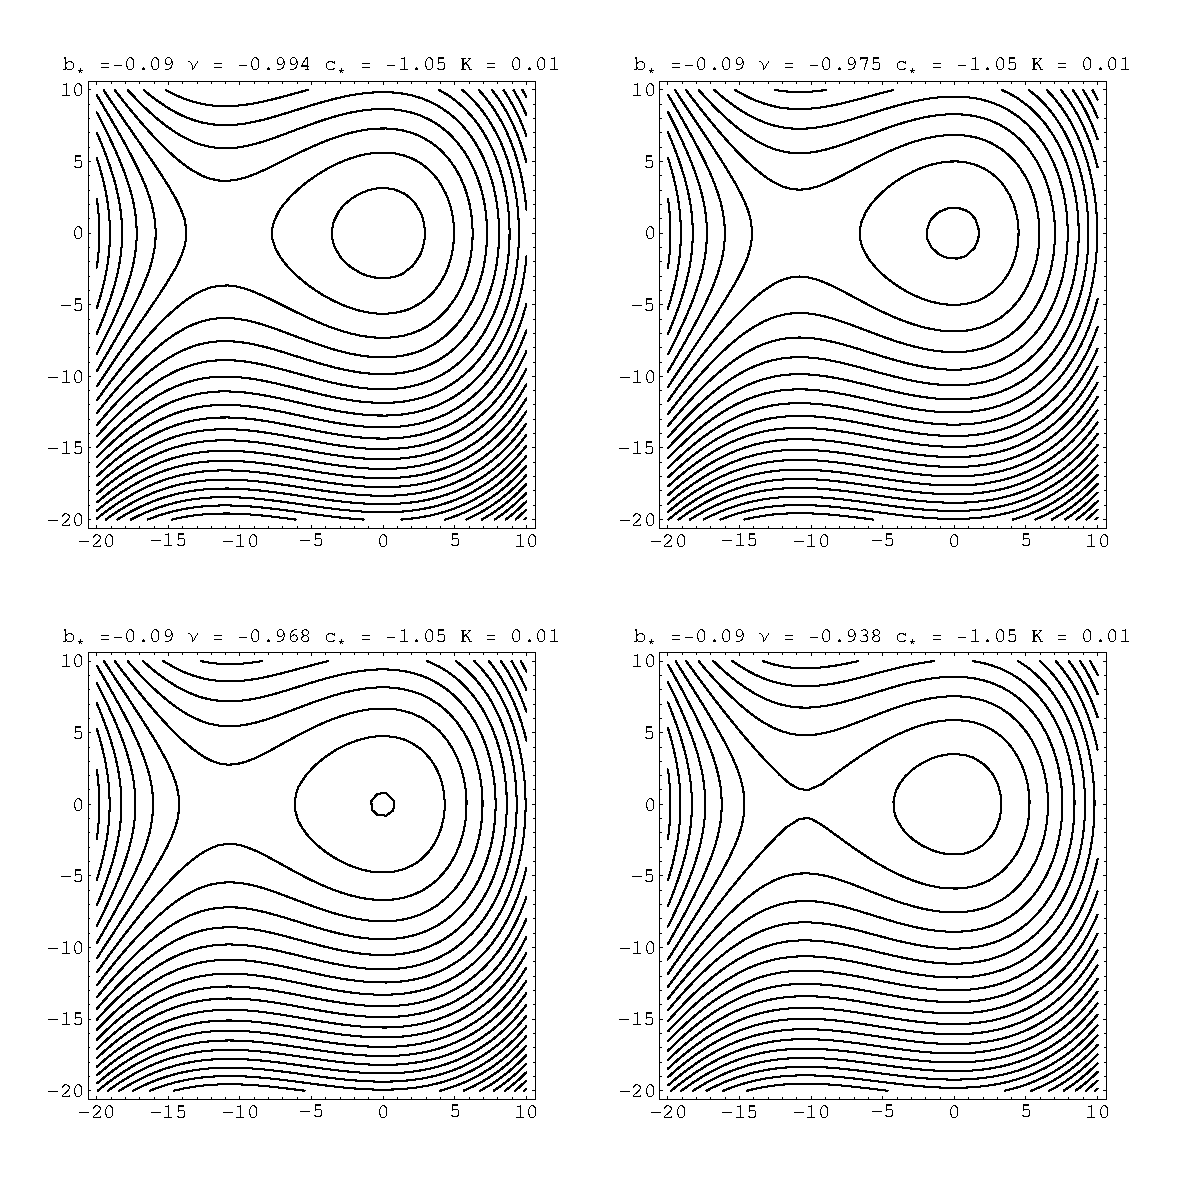
\includegraphics[width=1.0\textwidth]{figures/figure3-1a}  
\caption{Level curves of \eqref{eq:H2} corresponding to various values of H.}
\end{center}
\end{figure}
